\documentclass[]{amsart}

\usepackage{graphicx}

\title{A numerical Example on the idea of declustering}
\author{Keivan Hassani Monfared}
\address{k1monfared@gmail.com}

\begin{document}
\maketitle

\begin{abstract}
	A numerical example is shown to conceptualize the idea of declustering.
\end{abstract}

\section{Introduction}
	When a hierarchical clustering algorithm is used to cluster a graph, it sometimes happens that the subclusters of two previously separated clusters could be very close to each other. Here we show one example of such situation in graphs.
	
\section{A numerical example}
	Let $G$ be a weighted graph with the following adjacency matrix.
	
	\begin{center}
		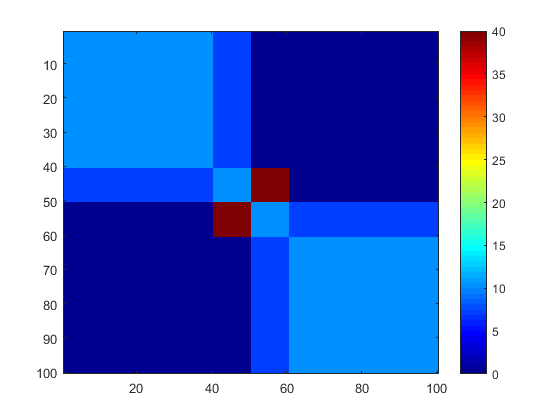
\includegraphics[width = .8\linewidth]{sample_graph}
	\end{center}
	
	Using the iterative Fiedler method we can break this into two (and three) and four clusters, as shown below. The method first breaks the graph right in the middle: first $50$ vertices are one cluster, and the rest are another cluster. Then one of the two clusters is broken down at $40$--$10$ ratio. And finally another cluster is broken down at $10$--$40$ ratio.
  	
	\begin{center}
		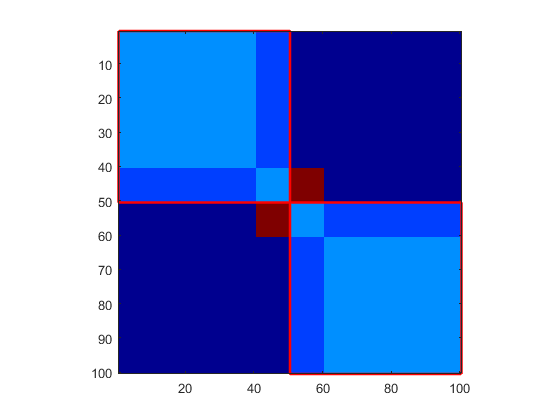
\includegraphics[width = .49\linewidth]{sample_graph_2c}
		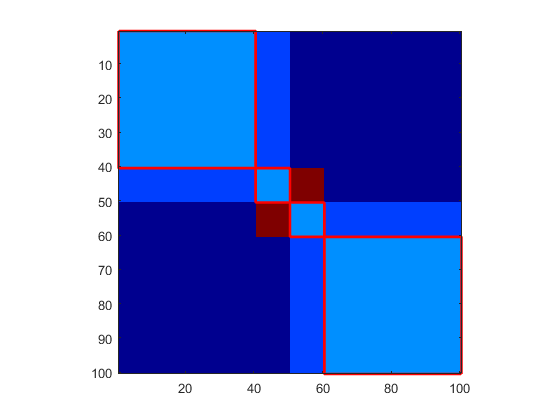
\includegraphics[width = .49\linewidth]{sample_graph_4c}
	\end{center}
	
	The intuitive to consider is that the middle two clusters, both of size $10$ were separated from each other because of the two big clusters of size $50$ in the first step. But now it seems like they can be glued back together, and they'll from a strong cluster. Let's see what will happen if we do this:
	
	\begin{center}
		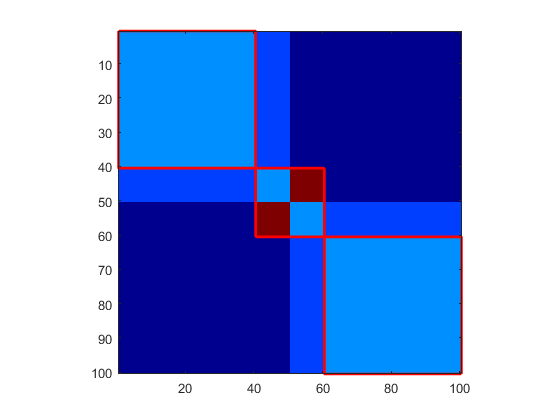
\includegraphics[width = .5\linewidth]{sample_graph_3c}
	\end{center}
	
	Here are the modularities of each clustering:
	
	\begin{center}
		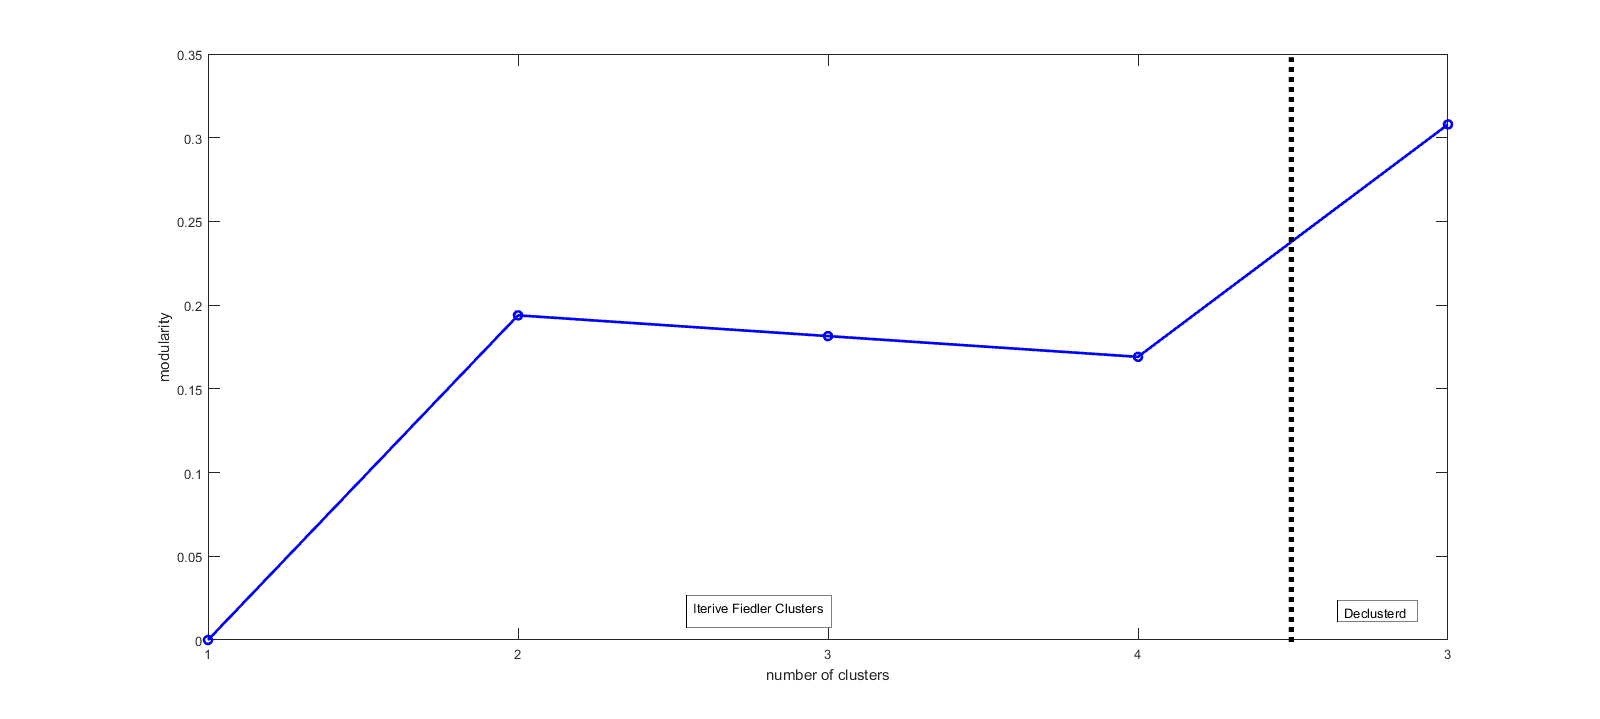
\includegraphics[width = \linewidth]{modularities}
	\end{center}
	
\section{Conclusion}
	The idea of declustering is essential in any clustering algorithm, and it needs to be implemented accordingly. 
\end{document}